\documentclass[tikz,border=10pt]{standalone}
\usepackage{tikz}
\usetikzlibrary{calc}

\begin{document}

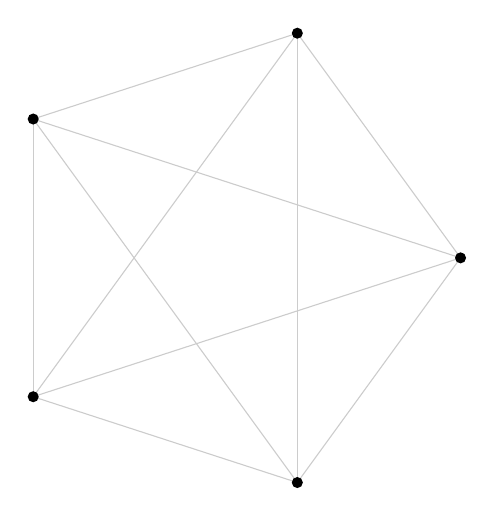
\begin{tikzpicture}
  % Define the radius of the hexagon
  \def\radius{3cm}

  % Define the vertices of the hexagon
  \foreach \i in {1,...,5} {
    \coordinate (V\i) at ({\radius*cos(72*(\i-1))}, {\radius*sin(72*(\i-1))});
  }

  % Draw edges for the complete graph K6
  \foreach \i in {1,...,5} {
    \foreach \j in {\i,...,5} % slight improvement suggested by Japheth Wood
      \draw[black!20!] (V\i) -- (V\j);
    }

  % Draw the vertices
  \foreach \i in {1,...,5} {
    \fill (V\i) circle (2pt);
  }

\end{tikzpicture}

\end{document}